\section{Thermal diffusion in a cube}

\noindent The purpose of this section is to draw an analogy between the equations encountered with infinite quantum wells (cf. Quantum Physics TD 1 which will soon be addressed) and those of thermal diffusion in a solid with homogeneous boundary conditions (as described below).
In both cases:

\begin{itemize}
    \item Solving so-called "transport" equations;
    \item Observing quantification of solutions, i.e., eigenmodes for temperature propagation in one case or probability of presence in the other.
\end{itemize}

\noindent Consider a solid of infinite height along $\vec{e_y}$ and of width $L$ along $\vec{e_x}$ in a liquid assumed to be infinite at temperature $T_f$, assumed constant and uniform.

\begin{figure}[htbp]
    \centering
    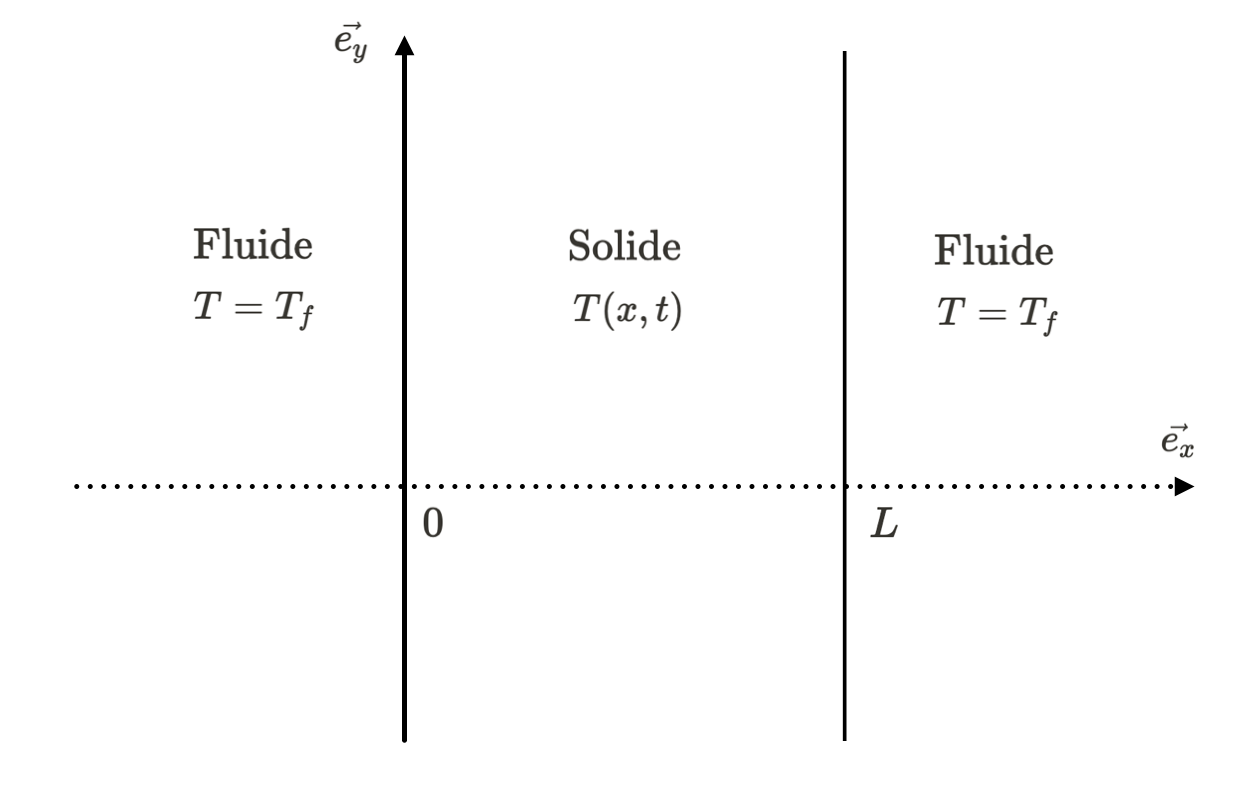
\includegraphics[width=0.5\textwidth]{TD1_2024_EN_Corr_TEX/Scheme_FR.png}
    \caption{Problem scheme}
    \label{fig:schema_diff_thermique}
\end{figure}

\noindent We seek to determine the behavior of the temperature $T(x,t)$ in the solid as a function of position $x$ and time $t$.
The differential equation satisfied by $\theta(x,t) = T(x,t) - T_f$ is \textbf{the heat equation}. It is given by:

\begin{equation}
\frac{\partial \theta}{\partial t} = D \nabla^2 \theta
\label{exocube}
\end{equation}

\noindent where $D = \displaystyle \frac{\lambda}{\rho c_P}$ is the thermal diffusivity of the solid, with $\lambda$ its thermal conductivity, $\rho$ its density, $c_P$ its specific heat capacity at constant pressure.\\ \\
\noindent \textbf{1.a)} By using the method of separation of variables, propose a form of the solution of equation (\ref{exocube}) and write the independent equations of time and space respectively. We will call the introduced constant $\displaystyle -\frac{1}{\tau}$.\\

\begin{breakbox}
    \noindent By separation of variables, $\theta(x,t) = \varphi(x)g(t)$. The equations are therefore as follows for $x \in [0,L]$ and $t > 0$:
    \\
    $$\boxed{
    \begin{cases}
        g'(t) + \frac{1}{\tau}g(t) = 0 \\
        \varphi''(x) + \frac{1}{\tau D}\varphi(x) = 0
    \end{cases},}$$
    \\
    with $\tau \in \mathbb{R}$.
\end{breakbox}

\medskip

\noindent \textbf{1.b)} Provide the boundary conditions satisfied by $\theta(x,t)$.\\

\begin{breakbox}
    \noindent In the fluid, the temperature is assumed constant and uniform, thus:
    $$\boxed{\theta(0,t) = \theta(L, t) = T_f - T_f = 0.}$$
\end{breakbox}

\medskip

\noindent \textbf{2)} Give the general form of the solution of the time-dependent equation. What is the sign of $-\frac{1}{\tau}$? To what is $\tau$ homogeneous?\\

\begin{breakbox}
    \noindent We have: $$\boxed{g(t) = A e^{-\frac{t}{\tau}} \text{ where }A \in \mathbb{R}.}$$ We necessarily have $\displaystyle \frac{1}{\tau} > 0$ for the solution not to diverge.
    $\tau$ is homogeneous to time.
\end{breakbox}

\medskip

\noindent \textbf{3.a)} Give the general form of the solution of the space-dependent equation.\\

\begin{breakbox}
    \noindent $$\boxed{\varphi(x) = C \cos(\sqrt{\frac{1}{\tau D}}x) + E \sin(\sqrt{\frac{1}{\tau D}}x) \text{ where } C, E \in \mathbb{R}.}$$
\end{breakbox}

\medskip

\noindent \textbf{3.b)} Simplify this expression using the boundary condition at $x = 0$.\\

\begin{breakbox}
    \noindent At $x=0$, we have $\varphi(0) = C = 0.$
    Thus, the solution is written as $\boxed{\varphi(x) = E \sin(\sqrt{\frac{1}{\tau D}}x)$ for $x \in \mathbb{R}}$.
\end{breakbox}

\medskip

\noindent \textbf{3.c)} Using the boundary condition imposed at $x=L$, give the allowed values for $\displaystyle \frac{1}{\tau}$.\\

\begin{breakbox}
    \noindent We note the appearance of eigenmodes, i.e., discrete values allowed for the constant $\displaystyle \frac{1}{\tau_n}$.
    Indeed, we have: $$\theta(L,t) = 0 \Rightarrow \sin(\sqrt{\frac{1}{\tau D}}L) = 0 \Rightarrow \sqrt{\frac{1}{\tau D}}L = n\pi \Rightarrow \boxed{\frac{1}{\tau_n} = \frac{D\pi^2}{L^2}n^2, \text{ where } n \in \mathbb{N}.}$$
\end{breakbox}

\medskip

\noindent \textbf{3.d)} What can be said about the general form of $\theta(x,t)$?\\

\begin{breakbox}
    \noindent The eigenmodes of the form $\displaystyle \varphi_n(x) = A_n \sin(\sqrt{\frac{1}{\tau_n D}}x)$ are such that:
    $$\theta_n(x,t) = A_n e^{-\frac{t}{\tau_n}} \sin(\sqrt{\frac{1}{\tau_n D}}x).$$ The general solution is therefore an infinite sum of these eigenmodes:
    $$\boxed{\theta(x,t) = \sum_{n=0}^{\infty} A_n e^{-\frac{t}{\tau_n}} \sin(\sqrt{\frac{1}{\tau_n D}}x) = \sum_{n=0}^{\infty} A_n e^{-\frac{D\pi^2}{L^2}n^2 t} \sin(\frac{n\pi}{L}x).}$$
\end{breakbox}

\medskip

\noindent In the case of a particle in an infinite quantum well of length $L$ with a potential (a case that will be addressed in Quantum Physics TD 1 to be held on Friday, 01/03), as in part \textbf{1.3} we seek the eigenmodes of the Schrödinger equation by separation of variables, to obtain the \underline{general} solutions of this equation that can be written as:
\begin{equation*}
    \psi(x, t) = \sum_{n=1}^{+\infty}\varphi_n(x) f_n(t).
\end{equation*}

\noindent We find that the solutions to the time-independent Schrödinger equation (i.e., the stationary states of the infinite well),
\begin{equation*}
    -\frac{\hbar^2}{2 m} \varphi_n^{''}(x) = E_n \varphi_n(x),
\end{equation*}

\noindent are functions $\displaystyle \varphi_n(x)=A\sin \left(\frac{n \pi x}{L}\right) \text{ with } n \in \mathbb{N}^{*}, \: A \in \mathbb{R}$. \\

\noindent Furthermore, the temporal dependence $f_n(t)$ of the eigenmode $n$ satisfies the equation:
\begin{equation*}
    f_n'(t) = -i\frac{E_n}{\hbar}f_n(t)
\end{equation*}
And is thus of the form $\displaystyle f_n(t) = B e^{-i\frac{E_n}{\hbar}t}, \: B \in \mathbb{R}$.
\noindent The normalization of each eigenmode requires $\displaystyle AB = \sqrt{\frac{2}{L}}$.
\noindent Thus, the general form $\psi(x,t)$ is:
$$\boxed{\psi(t, x) = \sum_{n=1}^{\infty} \sqrt{\frac{2}{L}} e^{-i\frac{E_n t}{\hbar}} \sin \left(\frac{n \pi x}{L}\right)}$$
with 
$
\displaystyle E_n = \frac{n^2 \hbar^2 \pi^2}{2mL^2}, \text{ where } n \in \mathbb{N^*}.
$\\

\noindent \textbf{4.a)} Let's push the analogy a little further. What is the physical significance of $\tau_n$? In the case of the infinite well, what quantity does $\frac{1}{\tau_n}$ compare to?\\

\begin{breakbox}
    \noindent $\tau_n$ is the characteristic time of the exponential decay of temperature in eigenmode $n$. In the case of the infinite quantum well, we identify $\displaystyle \frac{1}{\tau_n}$ with $\displaystyle i\frac{E_n}{\hbar}$.
\end{breakbox}

\medskip

\noindent \textbf{4.b)} How can we define the equivalent of thermal diffusivity $D$ in the case of the infinite quantum well? Can it be given a physical meaning?\\

\begin{breakbox}
    \noindent By expanding we have:
    $$i\frac{E_n}{\hbar} = i\frac{\hbar n^2 \pi^2}{2mL^2} = i\frac{\hbar}{2m} \frac{n^2\pi^2}{L^2}.$$
    By identifying terms in the exponential, we can define a "quantum diffusivity" $\displaystyle D_q = i\frac{\hbar}{2m}$, where $m$ is the mass of the particle.
    This quantity has no physical meaning, but allows to retrieve the expression of the eigenmodes of the infinite quantum well.
\end{breakbox}
